\documentclass[conference]{IEEEtran}
\usepackage{graphicx}
\usepackage{booktabs}
\usepackage{cite}
\usepackage{amsmath}
\usepackage{url}
\usepackage{multirow}
\usepackage[hidelinks]{hyperref}
\graphicspath{{figures/}}

\begin{document}

\title{AI-Assisted Web Application Penetration Testing:\\
Detecting and Classifying Web Attacks in Network Flows and HTTP Requests,\\
Validated Against OWASP ZAP}

\author{
\IEEEauthorblockN{Student One, Student Two, Student Three}
\IEEEauthorblockA{CSCI 561 Computer and Network Security\\
Group project, Topic 4: AI-Assisted Web Application Penetration Testing}
}

\maketitle

\begin{abstract}
Web applications remain the most attacked part of most organisations, and conventional
defences, such as signature rules in a web application firewall (WAF) or an active vulnerability
scanner, only recognise what they were written to recognise. We ask how effectively
machine learning (ML) can assist in detecting and classifying web-application attacks and how
it compares with conventional detection. We study the question at two levels. On network
flows (CIC-IDS2017), six ML models detect brute-force, XSS and SQL-injection flows with F1 up to
0.999, while a statistical threshold IDS detects none. A validity audit then shows that most
attack flows carry no payload and that a TCP fingerprint identifies the attacker. With both
confounds removed, F1 is still 0.96--0.97. On HTTP requests, models
over 35 URL, parameter, header and content features, plus nine engineered features, a
learned per-parameter profile, and a character n-gram model reach F1 0.993--0.995 on
de-duplicated HTTP CSIC 2010 and a macro-F1 of 0.999 for attack-type classification on
HttpParamsDataset. Every setting is chosen by inner cross-validation, and we test the results
against four traps: label permutation, near-duplicates, structural shortcuts and dataset
shift. The traps are real: models trained on one application flag most benign traffic of another,
and we find that three quarters of the unique ``normal'' requests in the newer SR-BH 2020 dataset
are scanner attacks or carry injection payloads. Finally, a prototype that scores individual parameter values
was tested live against OWASP Juice Shop with an OWASP ZAP active scan. It raised false alarms on
0.45\% of benign requests and detected 95\% of SQL-injection and 94\% of XSS payloads, against
73\% and 94\% for CRS-style signature rules, and it ranks the vulnerable endpoints that ZAP
confirmed.
\end{abstract}

\begin{IEEEkeywords}
web application security, penetration testing, intrusion detection, machine learning, SQL injection,
cross-site scripting, OWASP ZAP, dataset validity
\end{IEEEkeywords}

% ======================================================================
\section{Introduction}
Injection flaws and broken access control lead the OWASP Top~10~\cite{owasptop10}. Penetration
testers find them with scanners such as OWASP ZAP~\cite{zap}, which send crafted payloads and
confirm a vulnerability from the response. Defenders block them with WAF signature rule sets
such as the OWASP Core Rule Set (CRS)~\cite{crs}. Both depend on hand-written knowledge.
ML promises to learn the boundary between benign and malicious traffic from examples,
and near-perfect accuracies are routinely reported on public datasets~\cite{tadhani2024,yang2025}.
However, the security-ML literature warns that such numbers can be produced by spurious
correlations, data snooping and unrealistic evaluation~\cite{arp2022,sommer2010}.
This project therefore asks:
\emph{How effectively can AI/ML assist in detecting and classifying web-application attacks, and how
does its performance compare with conventional detection?}

Our contributions are:
(i)~a flow-level study on CIC-IDS2017 with six ML models, a conventional threshold IDS and a
validity audit;
(ii)~a request-level study on HTTP CSIC 2010, HttpParamsDataset and SR-BH 2020 that extracts
URL, parameter, header and content features, engineers new ones, learns an application profile
and tunes regularisation, all without touching the test data;
(iii)~four explicit checks of whether the accuracies are real;
(iv)~an AI-assisted assessment prototype with risk scoring, endpoint prioritisation and a
user interface; and
(v)~a live comparison with OWASP ZAP and signature rules against OWASP Juice Shop.

% ======================================================================
\section{Background and Related Work}
\subsection{Web attacks}
\emph{SQL injection} (SQLi, CWE-89) places attacker-controlled text into a database query, e.g.
\texttt{' OR 1=1--} in a login field. \emph{Cross-site scripting} (XSS, CWE-79) stores or reflects
script, e.g. \texttt{<script>}, into pages shown to other users. \emph{Path traversal} (CWE-22) and
\emph{OS command injection} (CWE-78) abuse file names and shell arguments. \emph{Authentication}
attacks guess or bypass credentials, and \emph{access-control} attacks reach objects or functions
of other users (insecure direct object references, missing function-level checks). The first
four leave a payload in the request. Brute force and access-control abuse usually do not: a
single password guess or a request for another user's basket looks like a legitimate request,
and only volume or authorisation context reveals it.

\subsection{Conventional detection}
Active scanners (ZAP, Burp Suite) inject payloads and confirm vulnerabilities from responses.
WAFs match payload patterns. The CRS groups its rules into families for SQLi (942xxx), XSS (941xxx),
local file inclusion (930xxx) and remote command execution (932xxx)~\cite{crs}. Signatures are precise but
brittle: adversarial rewriting evaded ML-based SQLi detectors in up to 100\% of attempts and
evaded all seven commercial WAF services tested~\cite{qu2024}, and Floris \emph{et al.} raised CRS
detection by up to 30\% with negligible false alarms by learning how to weight its rules~\cite{floris2025}.
Statistical anomaly detection~\cite{denning1987}, and per-parameter profiles of length and
character distribution for web requests~\cite{kruegel2003}, are the conventional techniques that
need no signatures.

\subsection{Machine learning for web attacks}
CIC-IDS2017~\cite{sharafaldin2018} is a standard benchmark, with broad ML comparisons in
\cite{maseer2021,kurniabudi2020}. Audits found that CICFlowMeter splits connections into spurious
payload-less flows and that labelling errors change measured performance~\cite{engelen2021,lanvin2023}.
At request level, Tadhani \emph{et al.}~\cite{tadhani2024} report 99.77\% accuracy on CSIC 2010
with a CNN-LSTM, and Yang \emph{et al.}~\cite{yang2025} report 90.9\% on CSIC 2010 and 92.2\% on
HttpParams with an autoencoder and an MLP. Earlier work learned from request strings with deep
models~\cite{liang2017} or from XSS payload features~\cite{mereani2018}.
LLM agents now automate parts of penetration testing~\cite{deng2024,shen2025}. Guo \emph{et al.}
show that LLM agents exploit known web vulnerabilities in up to 90\% of cases but recall only about 50\% of them during autonomous
reconnaissance~\cite{guo2026}. Our work targets that weak step: scoring traffic and pointing the
tester to the riskiest endpoints.

% ======================================================================
\section{Data}
\textbf{CIC-IDS2017 (flows).} We use the Thursday web-attack day, verified against published
label counts and SHA-256 hashes, and Monday (benign only) as an unseen day. After repairing labels,
removing undefined-rate flows, 6,052 exact duplicates and constant columns, and restricting to
port-80 flows (other ports let a model ``detect'' web traffic instead of attacks), 19,725 flows with
66 CICFlowMeter features remain: 17,582 benign, 1,470 brute force, 652 XSS and 21 SQLi.

\textbf{HTTP CSIC 2010 (requests).} The dataset holds 97,065 requests to an e-commerce
application~\cite{csic2010}. Of these, 64\% are exact duplicates. A random split would place copies of the same
request in training and test, so we keep 34,593 unique requests (46.1\% anomalous).

\textbf{HttpParamsDataset (payloads).} 31,067 parameter values labelled normal, SQLi, XSS,
command injection or path traversal, with an official train/test split~\cite{httpparams}. We remove
test payloads that also occur in training.

\textbf{SR-BH 2020 (requests).} 907,814 requests to an Internet-exposed WordPress server in July
2020, with CAPEC multi-labels~\cite{srbh2022}. Dictionary password guesses (CAPEC-16) are
content-identical to normal logins, so the 836 requests labelled only CAPEC-16 are removed. Manual
inspection of the 90,306 unique ``normal'' requests showed that 69,008 (76\%) are OWASP ZAP
scan traffic or carry injection characters, mostly in the URL path, e.g.
\texttt{/blog";cat /etc/passwd;"/wp-content} and ZAP's \texttt{zApPX} markers. We drop these
(we do not relabel them) using explicit, detector-independent criteria.

\textbf{Combined request dataset.} CSIC 2010 and the cleaned SR-BH 2020 are merged into one schema:
method, path, query, body, content type, a binary label, an attack type and the source. We
de-duplicate across sources and sample SR-BH 50/50 normal/attack, so that neither source dominates
and the source carries no label information.

% ======================================================================
\section{Method}
\subsection{Flow-level detectors}
Logistic regression (LR), linear SVM, random forest (RF), histogram gradient boosting, XGBoost~\cite{xgboost}
and an MLP are trained with class balancing; the linear models and the MLP get signed-log and standardised
features. The conventional baseline follows Denning~\cite{denning1987}: it learns each feature's benign
0.5--99.5th percentile range and raises an alarm when at least $m$ features are out of range, with $m$
chosen for a 1\% false-alarm budget.

\subsection{Request features}
Every value is URL-decoded up to twice, so that double-encoded payloads are seen. Headers that identify
a tool or a session (User-Agent, Cookie, Host, X-ZAP-Scan-ID, \dots) are never model input: a
detector must not learn to recognise the scanner instead of the attack. The 35 base features
follow the brief's four groups:
\emph{URL} (method, path length and depth, unusual characters, backup-file extensions, traversal),
\emph{parameters} (count, query/body length, longest and mean value, \%-encoding, double encoding),
\emph{headers} (special characters and attack keywords in content-bearing headers) and
\emph{content} (special characters, quotes, brackets, comment markers, character ratios, entropy, and
SQL, XSS, traversal, command and SSI/template keyword counts).
Nine \emph{engineered} features describe how a value is built: the longest run of special characters,
function-call patterns, character-class switches per character, encoding tricks (\texttt{0x}, \texttt{\&\#},
\texttt{char(}), mixed-case keywords (\texttt{SeLeCt}), keyword density, tokens, the non-alphanumeric
share and URLs inside values.
Finally, a \emph{learned application profile} in the spirit of Kruegel and Vigna~\cite{kruegel2003}
is fitted on benign training requests only. For every endpoint and parameter it learns the normal
value length, character set and character classes. A request is then described by an unseen
endpoint, unseen parameters, a length z-score, unseen characters and unseen character classes.

\subsection{Request models and regularisation}
LR, RF and XGBoost use the features. An NLP model, a TF-IDF of character 1--4-grams of the decoded request
followed by a linear SVM (``char-SVM''), learns payload fragments directly, and a \emph{hybrid} SVM combines
both. All preprocessing (scaling, log transform, profile, TF-IDF, feature selection) is part of a
scikit-learn pipeline~\cite{sklearn}, so it is re-fitted inside every training fold.
Hyperparameters are chosen by inner three-fold cross-validation on the training split only:
LR penalty (L2, elastic net, L1) and strength $C$ with an optional correlation filter;
RF depth, leaf size and features per split; XGBoost depth, minimum child weight, L1/L2 leaf
penalties, shrinkage and subsampling (30 random draws); and $C$ for the SVMs.
The conventional request baseline is a set of 31 signature rules modelled on the CRS families.

\subsection{Prototype}
The deployed analyser scores \emph{parameter values}, not whole requests. Each query, form, JSON,
unusual path segment and content-bearing header value is classified by an ensemble of a calibrated
char-SVM and XGBoost, both trained on HttpParamsDataset, into normal, SQLi, XSS, path traversal or
command injection. The most suspicious value gives the request's attack probability $p$ and class $c$.
Risk is $p\cdot s_c$ with severity $s_c$ (SQLi and command injection 1.0, path traversal 0.8, XSS 0.7),
mapped to High/Medium/Low. Each finding is explained by the signature rules that fired and by
features beyond the 99th percentile of benign values. Findings are grouped by endpoint, parameter
and class and ranked by maximum risk $\times \log(1+\text{requests})$. A Streamlit interface analyses
pasted requests, uploaded traffic (proxy logs, HAR, CSV, raw requests or access logs) and
CICFlowMeter files.

\subsection{Evaluation protocol}
CIC and CSIC use a stratified 80/20 held-out split plus stratified five-fold cross-validation
(seed 42). Robustness is tested with unseen attack types (leave one attack type out), timing evasion
(inter-arrival features scaled by 2--100$\times$), an unseen benign day and cross-dataset testing.
Four checks target false accuracy: \textbf{S1}, training on shuffled labels (must fall to chance);
\textbf{S2}, test requests that are near-duplicates of training requests (equal up to digits and case),
with re-scoring on novel requests only; \textbf{S3}, bootstrap 95\% confidence intervals; and
\textbf{S4}, a model that sees only request structure (method, lengths, counts) and no content.

\textbf{Lab.} On one machine, OWASP Juice Shop 20.3~\cite{juiceshop} runs behind a logging reverse proxy
on the loopback interface. Phase~A: 60 simulated shoppers browse, register, log in, fill baskets, post
reviews and feedback; one input in eight is benign but ``awkward'' (\texttt{o'neill}, \texttt{<3},
\texttt{50\% off}). Phase~B: ZAP 2.17 receives one example of every API endpoint seen in phase~A,
spiders, and runs a full active scan with the rule ID injected into every attack request. That
header gives per-request ground truth and is hidden from all detectors.
ZAP sends many requests without an attack payload (reflection markers such as \texttt{0W45pz4p},
numeric fuzzing, probes). We therefore also report recall on \emph{payload-bearing} requests, defined
by characters alone, as the CIC-IDS2017 audit's payload filter does for flows.

% ======================================================================
\section{Results}
\begin{table*}[t]
\centering
\caption{Main results. F1 on held-out test data unless stated; FPR = false-positive rate. All
request models use hyperparameters chosen by inner cross-validation on the training split.}
\label{tab:results}
\setlength{\tabcolsep}{3.6pt}\renewcommand{\arraystretch}{1.05}
\resizebox{\textwidth}{!}{%
\begin{tabular}{@{}llcccl@{}}
\toprule
Setting & Detector & F1 / macro-F1 & Recall & FPR & Note \\
\midrule
\multirow{4}{*}{\shortstack[l]{CIC-IDS2017 flows,\\ detection}}
 & XGBoost & 0.999 & 1.000 & 0.0003 & 5-fold CV F1 $0.998\pm0.001$ \\
 & Random forest & 0.993 & 0.986 & 0.0000 & \\
 & Threshold IDS (conventional) & 0.000 & 0.000 & 0.0068 & ROC-AUC 0.49 \\
 & XGBoost, audit setting S3 & 0.960 & 0.968 & 0.0006 & payload flows, no TCP fingerprint \\
CIC-IDS2017, attack type & XGBoost & 0.764 / 0.906 & -- & -- & macro-F1, all flows / S3 \\
\midrule
\multirow{6}{*}{\shortstack[l]{CSIC 2010 requests,\\ de-duplicated}}
 & Hybrid char n-grams + features & 0.995 & 0.993 & 0.0024 & 95\% CI [0.993, 0.997] \\
 & Char n-gram SVM (NLP) & 0.994 & 0.992 & 0.0035 & CV $0.996\pm0.001$ \\
 & XGBoost + learned profile & 0.993 & 0.989 & 0.0024 & without profile: CV 0.879 \\
 & Logistic regression + profile & 0.983 & 0.969 & 0.0024 & L1 penalty selected \\
 & Signature rules (conventional) & 0.339 & 0.204 & 0.0000 & \\
 & S1 shuffled labels (char-SVM) & -- & -- & -- & ROC-AUC 0.509 (chance) \\
HttpParams, attack type & Char n-gram SVM / signatures & 0.999 / 0.789 & -- & -- & macro-F1, 5 classes \\
\midrule
\multirow{3}{*}{\shortstack[l]{Juice Shop lab,\\ ZAP active scan}}
 & AI prototype & -- & 0.95 / 0.94 / 0.82 / 0.79 & 0.0045 & SQLi/XSS/trav./cmd, payload-bearing \\
 & Signature rules (CRS-style) & -- & 0.73 / 0.94 / 0.32 / 0.39 & 0.0000 & same requests \\
 & CSIC-trained XGBoost (whole request) & -- & 1.00 & 0.913 & fails on a new application \\
\bottomrule
\end{tabular}}
\end{table*}

\subsection{Flow level: ML versus a threshold IDS}
Table~\ref{tab:results} (top) summarises CIC-IDS2017. Every ML model detects web-attack flows
(cross-validated F1 0.96--0.998). XGBoost reaches 0.999 and detects all three attack types, including the
21 SQLi flows. The threshold IDS detects none at its 1\% false-alarm budget (ROC-AUC 0.49): attack flows
sit near the benign median on every metric, so no single-metric rule can separate them. Naming the attack
is harder: macro-F1 is at most 0.78, because brute-force and XSS flows are confused.

\textbf{Validity audit.} 91\% of the flows labelled as attacks carry no payload; they are TCP connection
fragments, as Engelen \emph{et al.} also found~\cite{engelen2021}. In addition, 94\% share the attacker
host's TCP initial window of 29,200, which identifies the machine rather than the attack. Fig.~\ref{fig:audit}
re-evaluates all models with each confound removed. Detection drops for the linear models (F1 0.74--0.81) but
stays high for the tree ensembles (RF 0.968, XGBoost 0.960, setting S3). Attack-type macro-F1 \emph{rises}
to 0.906, because an empty connection fragment cannot show which attack it belonged to.
Robustness is mixed. When SQLi is left out of training, XGBoost still detects 95\% of it, but RF only 43\%.
Slowing an attack down twofold breaks RF (recall 0.10), while LR stays at $\geq$0.95 even at 100$\times$.
On the unseen benign day, false alarms more than double for the linear models (to 2.4\%), but XGBoost
stays at 0.2\%.

\begin{figure*}[t]
\centering
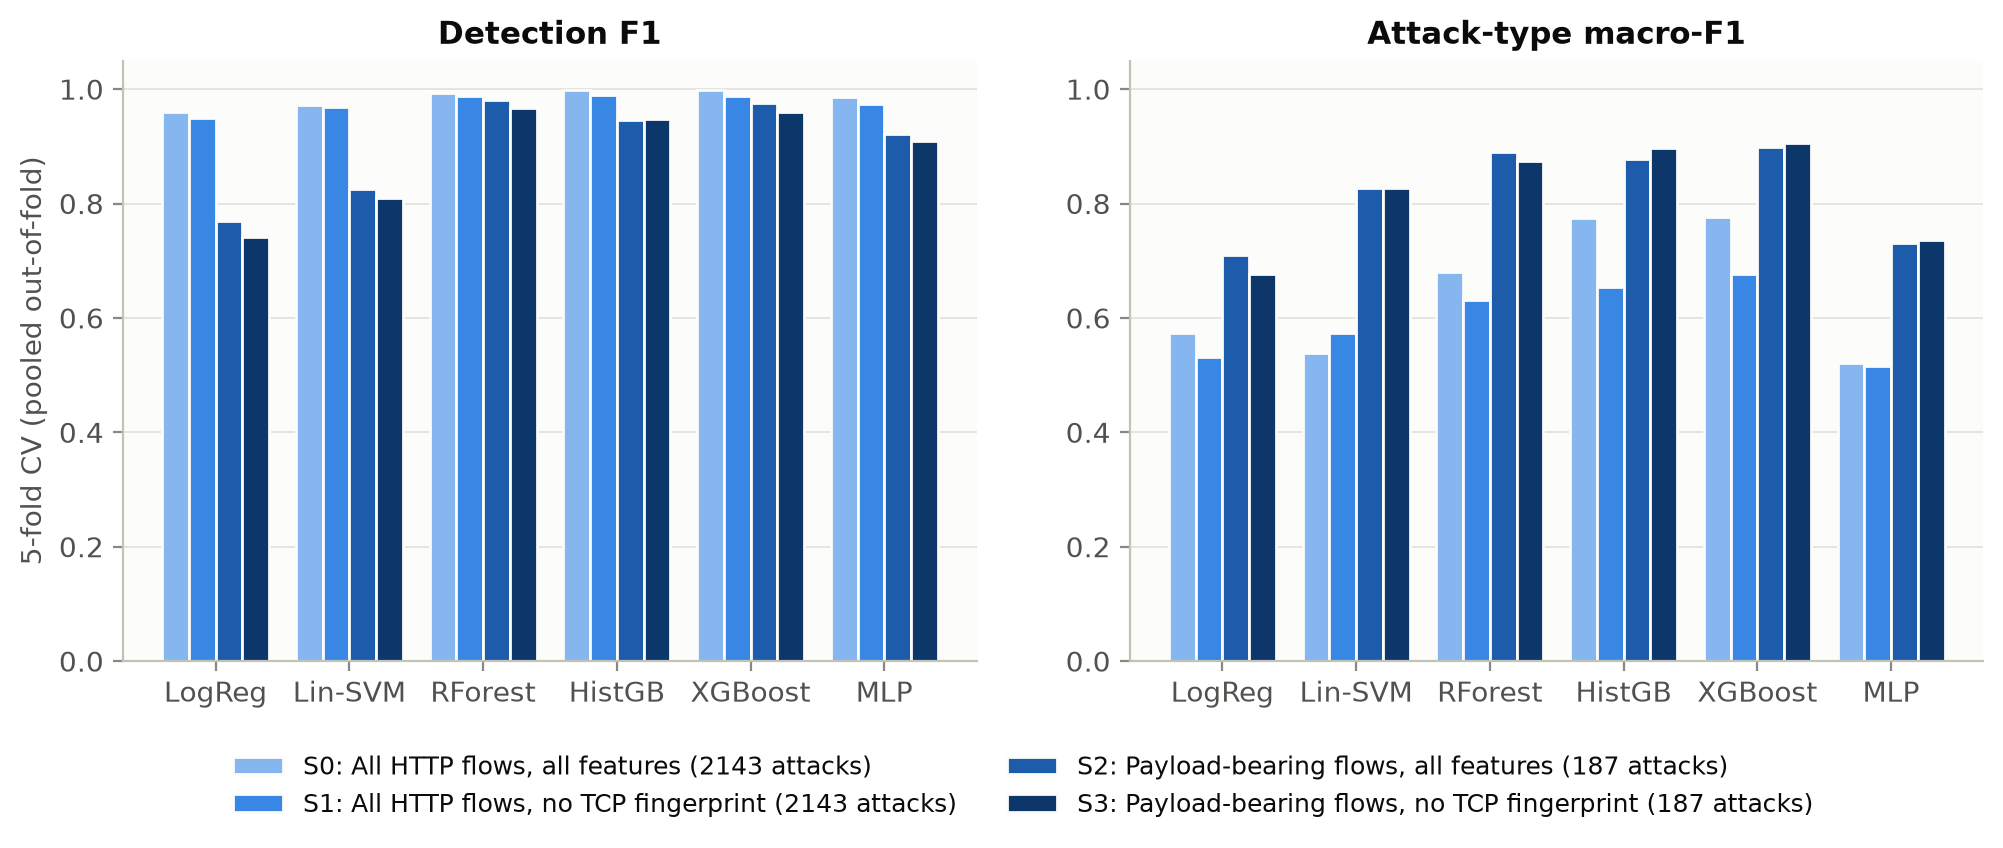
\includegraphics[width=0.86\textwidth]{fig05_validity_audit.png}
\caption{CIC-IDS2017 validity audit (5-fold CV). S0: all HTTP flows; S1: without the TCP-fingerprint
features; S2: payload-bearing flows only; S3: both. Detection survives the corrections for tree
ensembles; attack-type classification improves once payload-less fragments are removed.}
\label{fig:audit}
\end{figure*}

\subsection{Request level: features, profile and regularisation}
Fig.~\ref{fig:prep}(a) shows the feature ablation (five-fold CV on the CSIC training split). The
35 base features give F1 0.754 (LR) and 0.879 (XGBoost). The nine engineered features add nothing
on CSIC (0.749, 0.879), and nothing on HttpParams either (XGBoost macro-F1 0.948 vs.\ 0.946).
Their information is already carried by the keyword and character counts, and CSIC anomalies are
mostly malformed values rather than obfuscated payloads. The learned profile is decisive: F1 rises to 0.984 (LR) and 0.990
(XGBoost). Unseen characters, unseen endpoints and unseen parameters account for 97\% of XGBoost's
gain. The exploratory analysis explains why: four features, including both header features, are
constant on CSIC (every request carries the same headers), and profile features have the highest
mutual information with the label. The char-SVM reaches 0.984 without any hand-made features.

Regularisation was selected without the test set (Fig.~\ref{fig:prep}(b, c)). For LR, an L1 penalty
($C=0.1$) was selected; the training--test gap is 0.003, so LR does not overfit. XGBoost's training F1
reaches 1.0 from depth 6 onwards, while cross-validated F1 levels off at 0.990. The search therefore chose
strong leaf penalties ($\lambda=10$, $\alpha=1$, minimum child weight 3). Capping RF depth halved its
overfitting gap (0.016 to 0.008) and raised test F1 from 0.984 to 0.992. On the held-out test set the
best models reach F1 0.993--0.995 at an FPR of 0.24--0.35\% (Table~\ref{tab:results}), and five-fold
CV agrees to within 0.001. The CRS-style signatures are perfectly precise but find only 20\% of CSIC
anomalies, most of which carry no classic attack keyword.

\begin{figure*}[t]
\centering
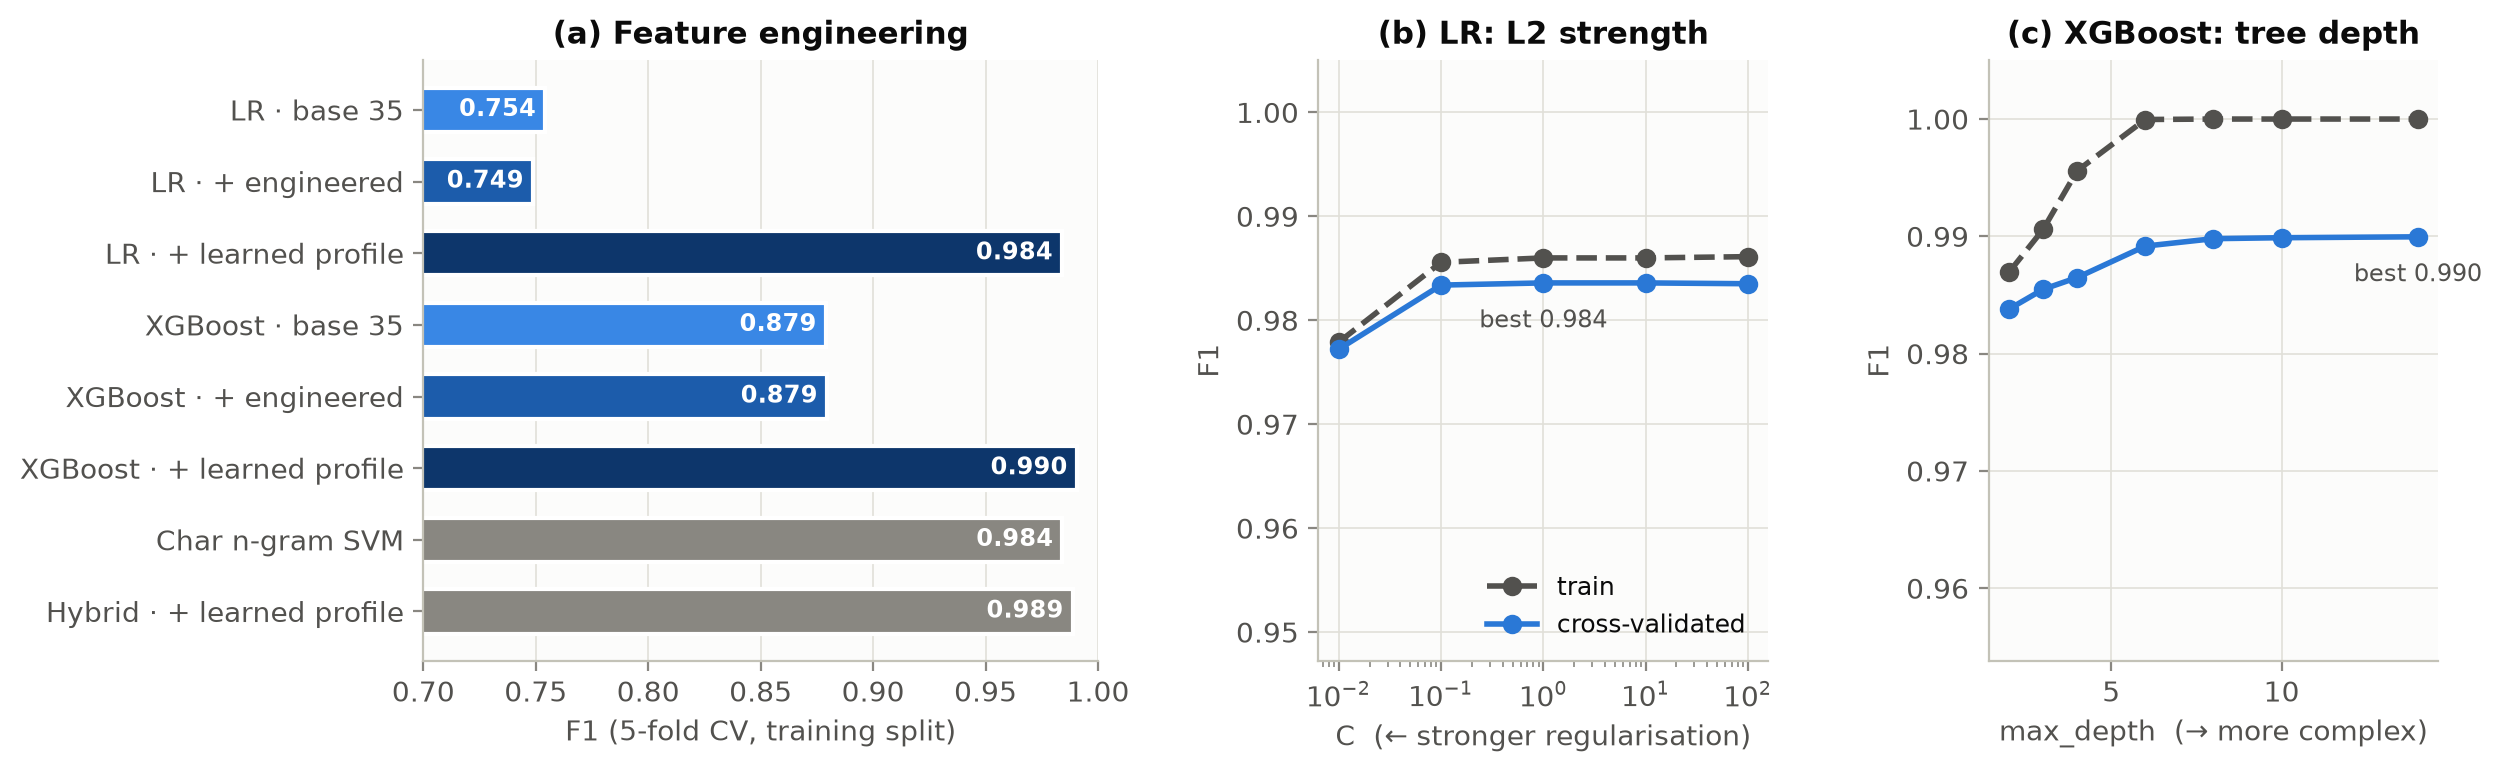
\includegraphics[width=0.94\textwidth]{fig11_preprocessing.png}
\caption{Feature engineering and regularisation on the CSIC 2010 training split. (a) Five-fold CV F1
by feature set: the learned per-parameter profile, not the engineered content features, closes the gap.
(b, c) Validation curves: training versus cross-validated F1 for LR as a function of the L2 strength and for
XGBoost as a function of tree depth.}
\label{fig:prep}
\end{figure*}

\textbf{Attack-type classification.} On the HttpParams test split, the char-SVM classifies the five
classes with macro-F1 0.999 (accuracy 99.97\%), the hybrid with 0.995 and XGBoost with 0.964. The
weakest class for the feature models is command injection (F1 0.87). The signatures reach 0.789:
their path-traversal and command rules miss 31--54\%.

\textbf{Are the accuracies real?} S1: trained on shuffled labels, the char-SVM falls to chance (ROC-AUC
0.509). XGBoost with the profile reaches 0.570, because a profile of novelty is partly informative even
without labels; this is not leakage. S2: 34.6\% of CSIC test requests have a near-duplicate in training
that differs only in digits or case. On the 4,524 novel test requests, F1 is still 0.990--0.992, so the models do not merely memorise.
S3: the 95\% confidence intervals of the three best models overlap ([0.991, 0.995], [0.992, 0.996],
[0.993, 0.997]), so their ranking is not significant. S4: request structure alone, without content,
already reaches F1 0.84 (ROC-AUC 0.94). CSIC is therefore easier than real traffic: its anomalies
differ in shape, and its normal values come from small dictionaries.

\textbf{Comparison with published results.} Under the protocol common in the literature (random split,
duplicates kept), our models reach 99.88\% accuracy on CSIC 2010, compared with 99.77\%~\cite{tadhani2024}
and 90.9\%~\cite{yang2025}. On HttpParams we reach 99.97\% accuracy, compared with 92.2\%~\cite{yang2025}.
De-duplication lowers our CSIC accuracy to 99.4\%. Splits and preprocessing differ between studies,
so these comparisons indicate rather than prove superiority.

\subsection{Generalisation: the trap of a single dataset}
Detectors trained on whole CSIC requests do not transfer. On HttpParams they flag 36--100\% of
\emph{benign} values, and in the Juice Shop lab they flag 91\% (XGBoost) and 99.9\% (char-SVM) of benign
shoppers. They have learned what normal looks like \emph{for that shop}.
The combined CSIC + SR-BH dataset (77,188 unique requests) tests this directly. One char-SVM trained on
both sources reaches F1 0.993 on each (FPR 0.38\% and 0.33\%). XGBoost without the profile reaches 0.945 and
0.972. With the learned profile, however, every model flags 57\% of SR-BH's benign requests: a public
WordPress site keeps producing endpoints and parameters that the profile has never seen, so ``new''
no longer means ``malicious''. This is the closed-world assumption that Sommer and Paxson warn
about~\cite{sommer2010}. Models trained on one source and tested on the other collapse (ROC-AUC 0.46--0.67): CSIC-trained models flag 96--100\% of SR-BH's benign requests, whereas the signature rules transfer (F1 0.75 on SR-BH at 0.06\% FPR). A classifier recognises the source of a request with 99.1\% accuracy, but because both sources were balanced, the source alone predicts nothing about the label (ROC-AUC 0.52).
This is why the prototype scores individual parameter values with models trained on payloads, not
whole requests.

\subsection{Live lab: AI prototype versus OWASP ZAP and signatures}
The lab logged 9,974 requests: 2,199 from benign shoppers, 412 from ZAP's exploration and 7,363 from
40 ZAP active-scan rules. The scan took 3.5 minutes. ZAP reported 42 distinct findings of 15 alert types,
including five High-risk ones: SQL injection in \texttt{POST /rest/user/login} (\texttt{email}) and
\texttt{GET /rest/products/search} (\texttt{q}), path traversal in \texttt{PUT /api/BasketItems/\{id\}}
(\texttt{quantity}), and external and off-site redirects. The rest are configuration findings (missing CSP,
version leaks, timestamps) that no traffic detector can report.

Fig.~\ref{fig:lab} compares the detectors on identical requests. The prototype raised false alarms on
0.45\% of benign requests (10 of 2,199), all on the shop's captcha field, whose negative answers such as
\texttt{-43} resemble numeric SQLi probes. On payload-bearing attack requests it detected 95\% of SQLi,
94\% of XSS, 82\% of path traversal, 79\% of command injection and 73\% of other injections. The signature
rules had no false alarms, but detected only 73\%, 94\%, 32\%, 39\% and 40\%. For the requests it
flagged, the prototype named the class ZAP's rule targeted 84\% of the time. The main confusion is
command-injection payloads read as SQLi (240 cases), because both use \texttt{;} and \texttt{|}.
Scoring took 0.71~ms per request.
The prototype's priority list puts SQLi on JSON parameters of \texttt{/api/Products}, \texttt{/api/Users},
\texttt{/api/Feedbacks} and \texttt{/rest/user/login} at the top. These are the endpoints ZAP attacked most
heavily, and they include the login SQLi that ZAP confirmed. For that finding, the prototype flagged 19
of ZAP's 24 attack requests (signatures: 11). For the confirmed path traversal it flagged 14 of 16
(signatures: 5).

\begin{figure*}[t]
\centering
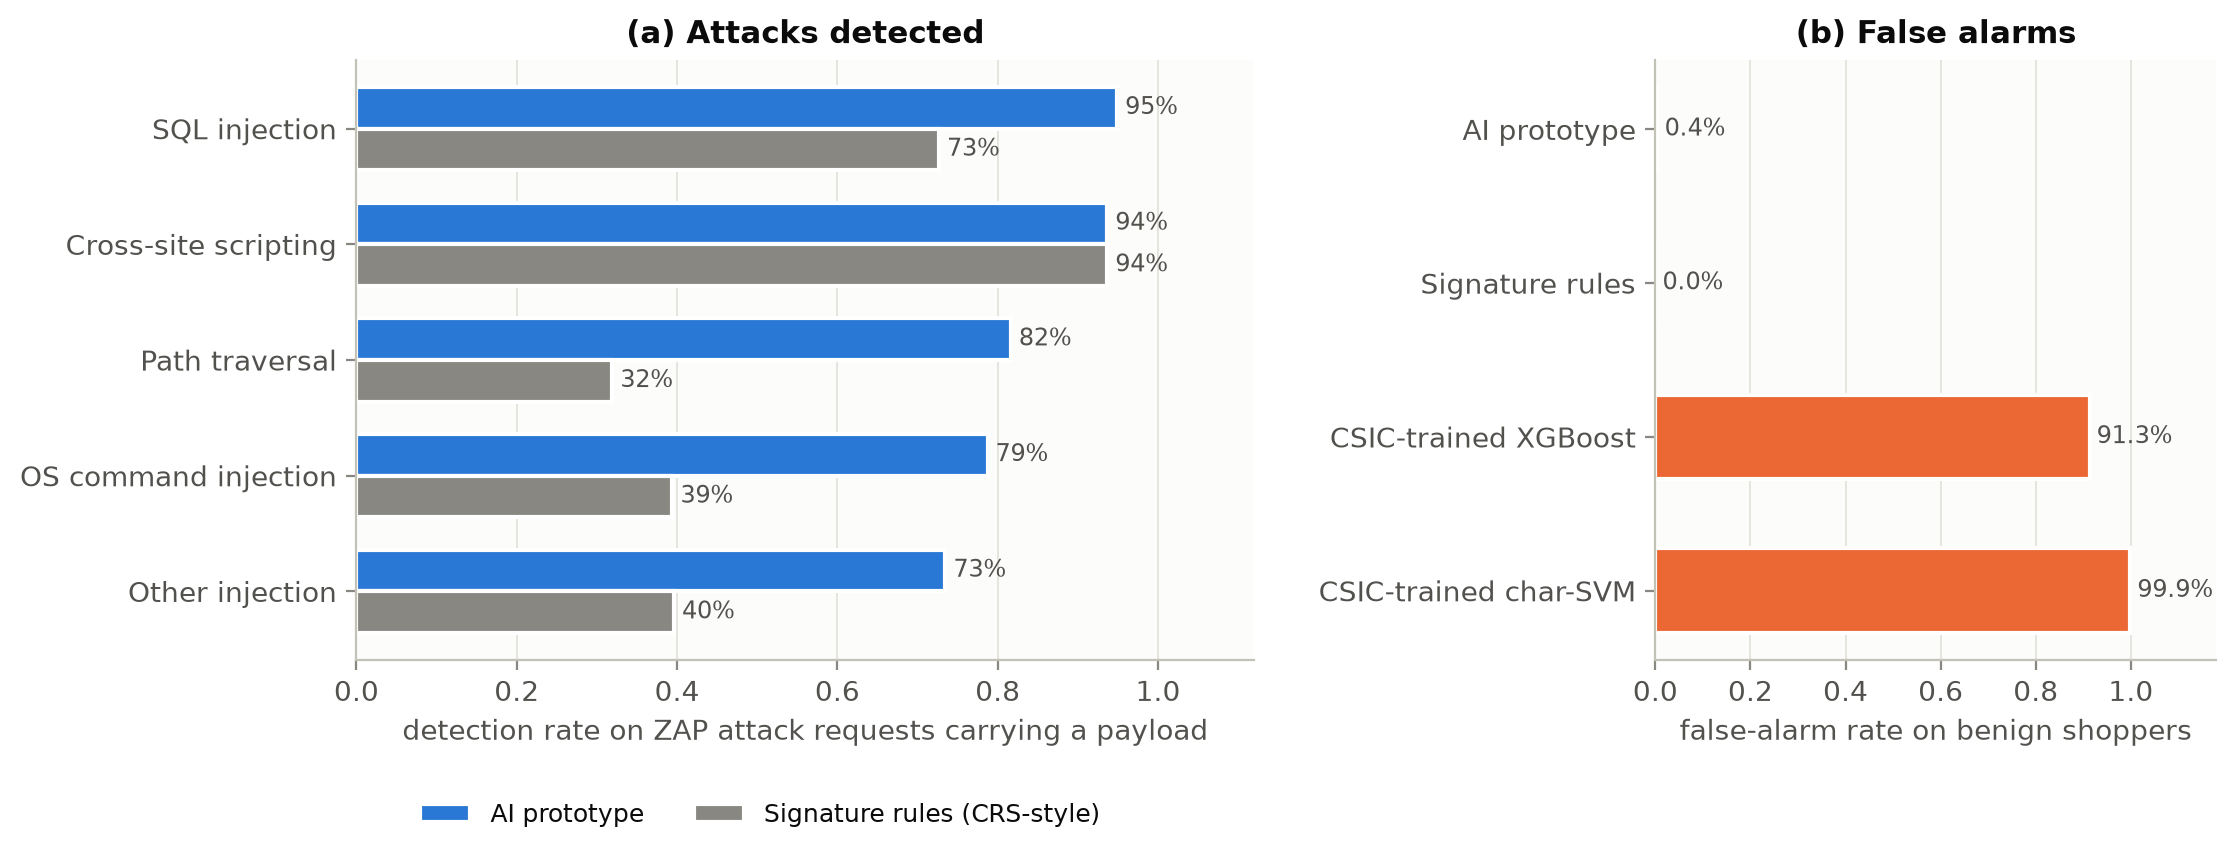
\includegraphics[width=0.9\textwidth]{fig12_lab.png}
\caption{Live lab on OWASP Juice Shop. (a) Detection rate on OWASP ZAP active-scan requests that carry an
injection payload, by the class of the ZAP rule that sent them. (b) False-alarm rate on 2,199 benign shopper
requests: models trained on another application's whole requests (CSIC) fail.}
\label{fig:lab}
\end{figure*}

% ======================================================================
\section{Discussion}
\textbf{AI versus conventional tools.} The conventional tools and the AI do different jobs. ZAP
\emph{confirms} vulnerabilities from responses and reports configuration weaknesses that are invisible in
traffic. The AI \emph{recognises attacks} in traffic, including attacks with no signature and attacks
that fail. In the lab it caught 1.3--2.6 times as many payload-bearing attacks as CRS-style signatures at a
0.45\% false-alarm rate, and its prioritisation pointed to the endpoints ZAP confirmed. Signatures
remain the better choice when no false alarm is acceptable. A practical workflow combines the two:
the AI triages traffic and ranks endpoints, and the scanner confirms them.

\textbf{False positives and negatives.} The prototype's false positives are short numeric values with a
leading minus. Its false negatives are mostly payload-free probes (reflection markers, numeric fuzzing,
which no content detector can flag) and command injections without shell keywords. The flow
models' errors concentrate on SQLi (21 flows) and on slowed-down attacks for the tree ensembles.

\textbf{Limitations.} Authentication brute force and access-control abuse leave no payload in a single
request. We exclude CAPEC-16 for this reason, and detecting them needs per-session volume or
authorisation context. CSIC 2010 is generated traffic, and SR-BH 2020 required heavy label cleaning,
which may have made its normal class easier. Each lab run used one application and one scanner, and an
adaptive attacker who rewrites payloads~\cite{qu2024} was not modelled. Deep sequence models and LLMs
were not evaluated.

\textbf{Ethics.} Only public datasets were used. The lab ran on the loopback interface against an
intentionally vulnerable application started and stopped by our script.

% ======================================================================
\section{Conclusion}
ML clearly outperforms conventional detection on both views of web traffic. It detects flow-level web
attacks that a statistical threshold IDS misses entirely, and in a live lab it finds 1.3--2.6 times more
attack payloads than CRS-style signatures, while classifying the attack and prioritising the vulnerable
endpoints. The accuracies, however, are only as real as the evaluation: duplicates, payload-less
flows, host fingerprints, closed-world profiles and mislabelled data each inflated or distorted results
in our study, and models that score 99.9\% on one dataset failed on another application. We therefore
recommend de-duplication, shuffled-label and near-duplicate checks, cross-dataset testing and a live lab
as standard practice. Future work: session-level features for brute force and access control, adversarial
training against payload rewriting~\cite{floris2025}, and pairing the analyser with an LLM agent that confirms
the endpoints it ranks highest.

% ======================================================================
\begin{thebibliography}{99}
\bibitem{owasptop10} OWASP Foundation, ``OWASP Top 10: 2021,'' 2021. [Online]. Available: \url{https://owasp.org/Top10/}
\bibitem{zap} OWASP Foundation, ``ZAP (Zed Attack Proxy),'' version 2.17, 2026. [Online]. Available: \url{https://www.zaproxy.org}
\bibitem{crs} OWASP Foundation, ``OWASP ModSecurity Core Rule Set.'' [Online]. Available: \url{https://coreruleset.org}
\bibitem{tadhani2024} J.~R. Tadhani, V.~Vekariya, V.~Sorathiya, S.~Alshathri, and W.~El-Shafai, ``Securing web applications against XSS and SQLi attacks using a novel deep learning approach,'' \emph{Scientific Reports}, vol.~14, 2024, doi: 10.1038/s41598-023-48845-4.
\bibitem{yang2025} J.~Yang, Y.~Wu, Y.~Yuan, H.~Xue, S.~Bourouis, M.~Abdel-Salam, S.~Prajapat, and L.~Y. Por, ``LLM-AE-MP: Web attack detection using a large language model with autoencoder and multilayer perceptron,'' \emph{Expert Systems with Applications}, vol.~274, art.~126982, 2025.
\bibitem{arp2022} D.~Arp \emph{et al.}, ``Dos and don'ts of machine learning in computer security,'' in \emph{Proc. 31st USENIX Security Symp.}, 2022.
\bibitem{sommer2010} R.~Sommer and V.~Paxson, ``Outside the closed world: On using machine learning for network intrusion detection,'' in \emph{Proc. IEEE Symp. Security and Privacy}, 2010, pp.~305--316.
\bibitem{qu2024} Z.~Qu, X.~Ling, T.~Wang, X.~Chen, S.~Ji, and C.~Wu, ``AdvSQLi: Generating adversarial SQL injections against real-world WAF-as-a-service,'' \emph{IEEE Trans. Inf. Forensics Security}, vol.~19, pp.~2623--2638, 2024, doi: 10.1109/TIFS.2024.3350911.
\bibitem{floris2025} G.~Floris, C.~Scano, B.~Montaruli, L.~Demetrio, A.~Valenza, L.~Compagna, D.~Ariu, L.~Piras, D.~Balzarotti, and B.~Biggio, ``ModSec-AdvLearn: Countering adversarial SQL injections with robust machine learning,'' \emph{IEEE Trans. Inf. Forensics Security}, 2025.
\bibitem{denning1987} D.~E. Denning, ``An intrusion-detection model,'' \emph{IEEE Trans. Softw. Eng.}, vol.~SE-13, no.~2, pp.~222--232, 1987.
\bibitem{kruegel2003} C.~Kruegel and G.~Vigna, ``Anomaly detection of web-based attacks,'' in \emph{Proc. 10th ACM Conf. Computer and Communications Security (CCS)}, 2003, pp.~251--261.
\bibitem{sharafaldin2018} I.~Sharafaldin, A.~H. Lashkari, and A.~A. Ghorbani, ``Toward generating a new intrusion detection dataset and intrusion traffic characterization,'' in \emph{Proc. 4th Int. Conf. Inf. Syst. Security and Privacy (ICISSP)}, 2018, pp.~108--116.
\bibitem{maseer2021} Z.~K. Maseer, R.~Yusof, N.~Bahaman, S.~A. Mostafa, and C.~F.~M. Foozy, ``Benchmarking of machine learning for anomaly based intrusion detection systems in the CICIDS2017 dataset,'' \emph{IEEE Access}, vol.~9, pp.~22351--22370, 2021.
\bibitem{kurniabudi2020} Kurniabudi, D.~Stiawan, Darmawijoyo, M.~Y. Bin Idris, A.~M. Bamhdi, and R.~Budiarto, ``CICIDS-2017 dataset feature analysis with information gain for anomaly detection,'' \emph{IEEE Access}, vol.~8, pp.~132911--132921, 2020.
\bibitem{engelen2021} G.~Engelen, V.~Rimmer, and W.~Joosen, ``Troubleshooting an intrusion detection dataset: The CICIDS2017 case study,'' in \emph{Proc. IEEE Security and Privacy Workshops (SPW)}, 2021, pp.~7--12.
\bibitem{lanvin2023} M.~Lanvin, P.-F. Gimenez, Y.~Han, F.~Majorczyk, L.~M\'e, and \'E.~Totel, ``Errors in the CICIDS2017 dataset and the significant differences in detection performances it makes,'' in \emph{Risks and Security of Internet and Systems (CRiSIS 2022)}, LNCS vol.~13857, Springer, 2023.
\bibitem{liang2017} J.~Liang, W.~Zhao, and W.~Ye, ``Anomaly-based web attack detection: A deep learning approach,'' in \emph{Proc. 6th Int. Conf. Network, Communication and Computing (ICNCC)}, ACM, 2017.
\bibitem{mereani2018} F.~A. Mereani and J.~M. Howe, ``Detecting cross-site scripting attacks using machine learning,'' in \emph{Advances in Intelligent Systems and Computing}, vol.~723, Springer, 2018, pp.~200--210.
\bibitem{deng2024} G.~Deng \emph{et al.}, ``PentestGPT: Evaluating and harnessing large language models for automated penetration testing,'' in \emph{Proc. 33rd USENIX Security Symp.}, 2024, pp.~847--864.
\bibitem{shen2025} X.~Shen, L.~Wang, Z.~Li, Y.~Chen, W.~Zhao, D.~Sun, J.~Wang, and W.~Ruan, ``PentestAgent: Incorporating LLM agents to automated penetration testing,'' in \emph{Proc. ACM Asia Conf. Computer and Communications Security (ASIA CCS)}, 2025, doi: 10.1145/3708821.3733882.
\bibitem{guo2026} Y.~Guo, L.~Yu, S.~Li, M.~Zhou, and G.~Chu, ``Decoupling reconnaissance and exploitation: Measuring the capability boundaries of LLM-based web penetration testing,'' in \emph{Proc. ICIC 2026}, LNCS vol.~16652, Springer, 2026, pp.~607--618.
\bibitem{csic2010} C.~Torrano Gim\'enez, A.~P\'erez Villegas, and G.~\'Alvarez Mara\~n\'on, ``HTTP data set CSIC 2010,'' Spanish National Research Council (CSIC), 2010.
\bibitem{httpparams} Morzeux, ``HttpParamsDataset,'' GitHub repository, 2016. [Online]. Available: \url{https://github.com/Morzeux/HttpParamsDataset}
\bibitem{srbh2022} T.~Sureda Riera, J.~R. Bermejo Higuera, J.~Bermejo Higuera, J.~A. Sicilia Montalvo, and J.~J. Mart\'inez Herr\'aiz, ``A new multi-label dataset for web attacks CAPEC classification using machine learning techniques,'' \emph{Computers \& Security}, vol.~120, art.~102788, 2022, doi: 10.1016/j.cose.2022.102788.
\bibitem{xgboost} T.~Chen and C.~Guestrin, ``XGBoost: A scalable tree boosting system,'' in \emph{Proc. 22nd ACM SIGKDD}, 2016, pp.~785--794.
\bibitem{sklearn} F.~Pedregosa \emph{et al.}, ``Scikit-learn: Machine learning in Python,'' \emph{J. Mach. Learn. Res.}, vol.~12, pp.~2825--2830, 2011.
\bibitem{juiceshop} OWASP Foundation, ``OWASP Juice Shop,'' version 20.3. [Online]. Available: \url{https://owasp.org/www-project-juice-shop/}
\end{thebibliography}

\end{document}
